\chapter{Existující řešení}
Existujících implementací je na síťovém trhu celá řada, nicméně ne každé řešení je vhodné pro potřeby předmětu Y36PSI.

\section{Cisco Packet Tracer}
Asi nejznámějším simulátorem směrovačů cisco je Packet Tracer \cite{cisco:pt} od firmy Cisco Systems. Program slouží k~simulaci síťového provozu počítačových sítí založených na hardwaru od Cisco Systems. Packet Tracer umožňuje vizualizaci provozu sítě, konfiguraci síťových prvků v~grafickém i~textovém módu. Program obsahuje velmi málo odchylek od skutečného cisco směrovače. Packet Tracer je dostupný pro platformy Windows i Linux zdarma pro všechny členy Cisco Networking Academy. To je zároveň velkou nevýhodou, protože licence neumožňuje jiné použití, proto je tedy Paket Tracer ve škole nepoužitelný.

\begin{figure}[h]
\begin{center}
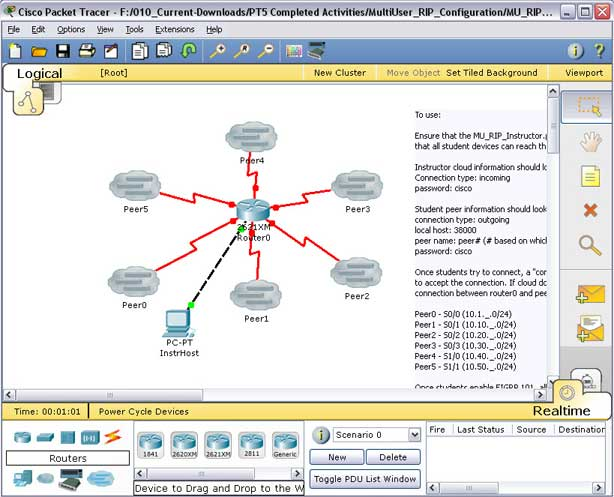
\includegraphics[width=7cm]{figures/r_cpt}
\caption{Cisco Packet Tracer}
\label{fig:r_cpt}
\end{center}
\end{figure}

\section{OMNeT++ simulátor} 
Simulační systém OMNeT++ \cite{reserse:omnet_hp} je velmi propracovaný nástroj pro simulaci prakticky čehokoliv. OMNeT++ je postaven na modulární architektuře, takže při správných knihovnách (modulech) může simulovat počítačovou síť. Systém dokáže simulovat Cisco IOS i počítač postavený na linuxu. Aplikace je komplikovaná a představu jednoduchého programu pro výuku studentů spíše nesplňuje.

Více se tímto simulátorem zabýval Bc. Jan Michek ve~své diplomové práci Emulátor počítačové sítě \cite{reserse:omnet_dp}.

\begin{figure}[h]
\begin{center}
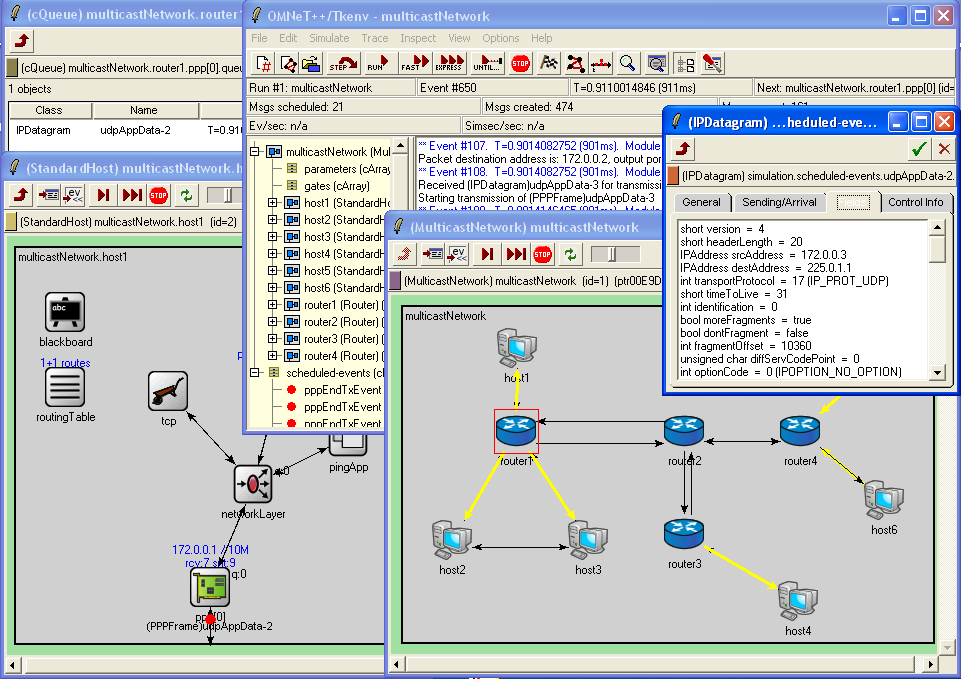
\includegraphics[width=7cm]{figures/r_omnet}
\caption{OMNeT++ simulátor}
\label{fig:r_omnet}
\end{center}
\end{figure}


\section{Simulation Toolkit 7.0} 
Simulation Toolkit 7.0 \cite{reserse:adventnet} je grafický simulátor pro testování a výuku různých síťových aplikací. Simulation Toolkit umožňuje simulaci více než 50000 SNMP služeb (v1, v2c, v3) TL1\footnote{Transaction Language 1}, TFTP\footnote{Trivial File Transfer Protocol }, FTP\footnote{File Transfer Protocol}, Telnet a Cisco IOS na jediném počítači. Software je nabízen pod shareware licencí a je dostupný pro operační systémy Windows, Linux i Unix. Za poskytnutí osobních údajů lze stáhnout plně funkční zkušební verzi na 30 dní. Plná časově neomezená verze stojí od \$995 do \$14995 \footnote{k~datu 23.5.2010}.


\section{Boson NetSim Network Simulator} 
Boson NetSim Network Simulator \cite{reserse:boson} je aplikace pro simulaci síťového hardwaru a softwaru a je designován jako výuková pomůcka pro začínající administrátory Cisco IOS. Systém dokáže simulovat více než 40 různých síťových prvků od firmy Cisco Systems. Simulátor obsahuje grafický i textový konfigurační režim sítí. Program je dostupný pro Windows, Linux i Solaris. Podobně jako Simulation Toolkit i tento software je nabízen ve zkušební verzi na 30 dní. Plná časově neomezená verze stojí od \$99 do \$349 \footnote{k~datu 23.5.2010}.

\begin{figure}[h]
\begin{center}
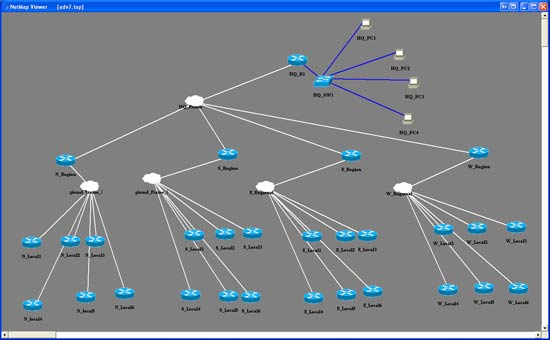
\includegraphics[width=7cm]{figures/r_boson}
\caption{Boson NetSim Network Simulator}
\label{fig:r_boson}
\end{center}
\end{figure}

\section{Dynamips Cisco 7200 Simulator}
Dynamips Cisco 7200 Simulator \cite{reserse:dynamips} je program napsaný Christophem Fillotem za účelem emulace Cisco směrovačů. Dynamips funguje na platformách Linux, Mac OS X, Windows a emuluje hardware Cisco směrovačů tak, že se načte obraz originálního Cisco IOS do emulátoru. Program tedy umožňuje využívat veškeré funkce Cisco IOS. Program je licencován pod GNU GPL\footnote{licence pro svobodný software}, ale obraz IOSu není bohužel volně k~dispozici. Tudíž lze program legálně používat jen jako účastník kurzu CNA\footnote{Cisco Networking Academy}, to ale studenti obvykle nejsou, proto tento software také není vhodný pro výuku.

\begin{figure}[h]
\begin{center}
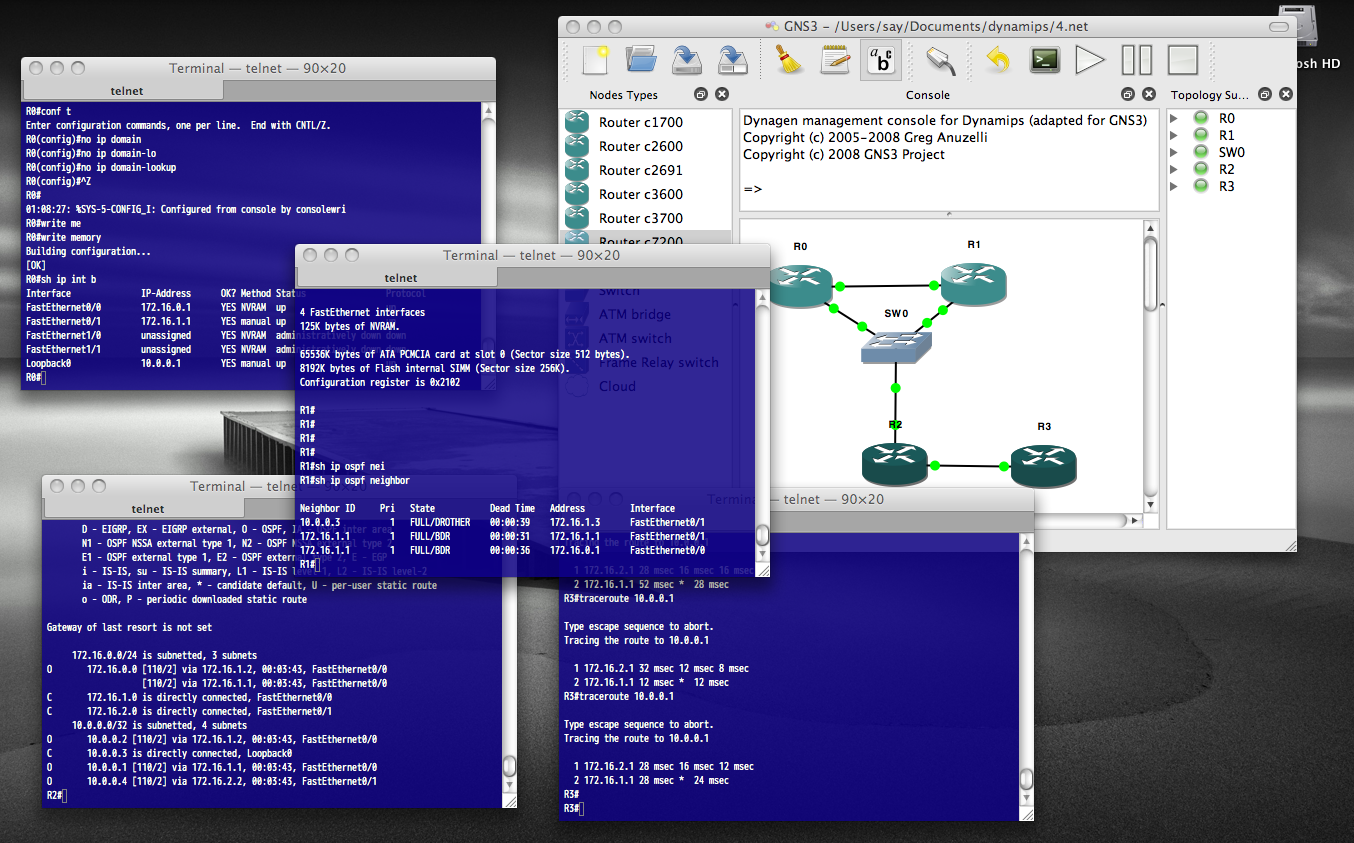
\includegraphics[width=7cm]{figures/r_dynamips}
\caption{Dynamips Cisco 7200 Simulator}
\label{fig:r_dynamips}
\end{center}
\end{figure}

\newpage

\section{Virtuální laboratoř počítačových sítí VirtLab}
Projekt VirtLab \cite{reserse:virtlab} zpřístupňuje laboratorní prvky pro praktickou výuku počítačových sítí vzdáleně prostřednictvím internetu. Studenti ostravské VŠB-TU\footnote{Vysoká škola báňská - Technická univerzita Ostrava} mají možnost si rezervovat pomocí webového rozhraní laboratorní síťové prvky na určitý časový interval a poté k~nim přistupovat přes webový prohlížeč pomocí Java appletů. Propojení síťových prvků se provede automaticky dle zvolené úlohy. Dle mého názoru je to systém velmi ambiciózní, nicméně pro výuku Y36PSI nepoužitelný\footnote{Za předpokladu že ČVUT nenaváže spolupráci s~VŠB-TU Ostrava.}.




